%Copyright 2014 Jean-Philippe Eisenbarth
%This program is free software: you can 
%redistribute it and/or modify it under the terms of the GNU General Public 
%License as published by the Free Software Foundation, either version 3 of the 
%License, or (at your option) any later version.
%This program is distributed in the hope that it will be useful,but WITHOUT ANY 
%WARRANTY; without even the implied warranty of MERCHANTABILITY or FITNESS FOR A 
%PARTICULAR PURPOSE. See the GNU General Public License for more details.
%You should have received a copy of the GNU General Public License along with 
%this program.  If not, see <http://www.gnu.org/licenses/>.

%Based on the code of Yiannis Lazarides
%http://tex.stackexchange.com/questions/42602/software-requirements-specification-with-latex
%http://tex.stackexchange.com/users/963/yiannis-lazarides
%Also based on the template of Karl E. Wiegers
%http://www.se.rit.edu/~emad/teaching/slides/srs_template_sep14.pdf
%http://karlwiegers.com
\documentclass{scrreprt}
\usepackage{listings}
\usepackage{underscore}
\usepackage[bookmarks=true]{hyperref}
\usepackage[utf8]{inputenc}
\usepackage{multirow}
\usepackage[table,xcdraw]{xcolor}
\usepackage[english]{babel}
\usepackage{graphicx}
\usepackage{caption}
\usepackage{subcaption}
\usepackage{wrapfig}
\usepackage[toc,xindy]{glossaries}
\usepackage{verbatim}
\usepackage{hyperref}
\usepackage[toc]{appendix}
\usepackage{booktabs}
\usepackage{amsmath}
\usepackage{grffile}
\newcommand{\addcustomplot}[4]{	
	{
		%\pgfplotstablegetcolsof{#}
		\addplot[scatter, color=#2,
		scatter/@pre marker code/.style={/tikz/mark size=2.0pt},
		scatter/@post marker code/.style={},
		line width = 1.5pt
		]
		table[x index=0,y index=#3, col sep=comma] {#1};
		\addlegendentryexpanded{#4}
	}
}

\newcommand{\addcustomybarplot}[4]
{
	\addplot[black,pattern color=#3,fill=#3,pattern=north east lines]  table[x index=0,y index=#2,col sep=comma]{#1};
	\addlegendentryexpanded{#4};
}


\newcommand{\plotfile}[1]{
	\pgfplotstableread{#1}{\table}
	\pgfplotstablegetcolsof{#1}
	\pgfmathtruncatemacro\numberofcols{\pgfplotsretval-1}
	\pgfplotsinvokeforeach{1,...,\numberofcols}{
		\pgfplotstablegetcolumnnamebyindex{##1}\of{\table}\to{\colname}
		\addplot table [y index=##1] {#1}; 
		\addlegendentryexpanded{\colname}
	}
}

\newcommand{\stencilpt}[4][]{\node[circle,draw,inner sep=0.1em,minimum size=0.8cm,font=\tiny,#1] at (#2) (#3) {#4}}


\lstset{
	basicstyle=\ttfamily\footnotesize,
	frame=single,
	breaklines=true,
	postbreak=\raisebox{0ex}[0ex][0ex]{\ensuremath{\color{red}\hookrightarrow\space}}
}


% Define block styles
\tikzstyle{decision} = [diamond, draw, fill=blue!20, 
text width=4.5em, text badly centered, node distance=3cm, inner sep=0pt]
\tikzstyle{block} = [rectangle, draw, fill=blue!20, 
 text centered, rounded corners, minimum height=4em, node distance=3cm]
\tikzstyle{line} = [draw, -latex']
\tikzstyle{cloud} = [draw, ellipse,fill=red!20, node distance=3cm,
minimum height=2em]
\hypersetup{
    bookmarks=false,    % show bookmarks bar?
    pdftitle={Level Test Case - System},    % title
    pdfauthor={Mateusz Gasior},                     % author
    pdfsubject={TeX and LaTeX},                        % subject of the document
    pdfkeywords={TeX, LaTeX, graphics, images}, % list of keywords
    colorlinks=true,       % false: boxed links; true: colored links
    linkcolor=blue,       % color of internal links
    citecolor=black,       % color of links to bibliography
    filecolor=black,        % color of file links
    urlcolor=purple,        % color of external links
    linktoc=page            % only page is linked
}%
\def\myversion{1.0 }
\date{}

\loadglsentries{others/glossary}
\makeglossaries

%\title

\begin{document}

\begin{flushright}
    \rule{16cm}{5pt}\vskip1cm
    \begin{bfseries}
        \Huge{LEVEL TEST\\ DESIGN}\\
        \vspace{1.9cm}
        for\\
        \vspace{1.9cm}
	    Supercomputer Simulation Tool\\
        \vspace{1.9cm}
        \LARGE{Version \myversion approved}\\
        \vspace{1.9cm}
        Prepared by Mateusz Gasior\\
        \vspace{1.9cm}
        Cranfield University\\
        \vspace{1.9cm}
        \today\\
    \end{bfseries}
\end{flushright}

\tableofcontents

\chapter*{Revision History}

\begin{center}
    \begin{tabular}{|c|c|c|c|}
        \hline
	    Name & Date & Description & Version\\ \hline
	    Mateusz Gasior & \emph{25-12-2016} & Skeleton of document. & 0.1 \\ \hline
	    Mateusz Gasior & \emph{04-01.2017} & Described level test case & 1.0 \\
        \hline
    \end{tabular}
\end{center}


\chapter{Introduction} \label{chp:introduction}

\section{Document identifier} \label{s:introduction:document-identifier}
	\begin{comment}
		$<$Uniquely identify a version of the document by including information such as the date of issue, the issuing organization, the author(s), the approval signatures (possibly electronic), and the status/version (e.g., draft, reviewed, corrected, or final). Identifying information may also include the reviewers and pertinent managers. This information is commonly put on an early page in the document, such as the cover page or the pages immediately following it. Some organizations put this information at the end of the document. This information may also be kept in a place other than in the text of the document (e.g., in the configuration management system or in the header or footer of the document).$>$
	\end{comment}
	\textsc{Document version: } 1.0 \\
	\textsc{Date of issue:} \today \\
	\textsc{Issuing organization:} Cranfield University \\
	\textsc{Authors: } Mateusz Gasior \\
	\textsc{Status: } Final \\

\section{Scope} \label{s:introduction:scope}
	\begin{comment}
		$<$Describe the purpose, goals, and scope of the system/software test effort. Include a description of any
		tailoring of this standard that has been implemented. Identify the project(s) for which the Plan is being
		written and the specific processes and products covered by the test effort. Describe the inclusions,
		exclusions, and assumptions/limitations. It is important to define clearly the limits of the test effort for
		any test plan. This is most clearly done by specifying what is being included (inclusions) and equally
		important, what is being excluded (exclusions) from the test effort. For example, only the current new
		version of a product might be included and prior versions might be excluded from a specific test effort.
		In addition, there may be gray areas for the test effort (assumptions and/or limitations) where
		management discretion or technical assumptions are being used to direct or influence the test effort.
		For example, system subcomponents purchased from other suppliers might be assumed to have been
		tested by their originators, and thus, their testing in this effort would be limited to only test the features
		used as subcomponents in the new system.If the development is based on a “waterfall” methodology, then each level of the test will be executed
		only one time. However, if the development is based on an iterative methodology, then there will be
		multiple iterations of each level of test. For example, component testing may be taking place on the
		most recent iteration at the same time that acceptance testing is taking place on products that were
		developed during an earlier iteration.
		The test approach identifies what will be tested and in what order for the entire gamut of testing levels
		(component, component integration, system, and acceptance). The test approach identifies the rationale
		for testing or not testing, and it identifies the rationale for the selected order of testing. The test
		approach describes the relationship to the development methodology. The test approach may identify
		the types of testing done at the different levels. For example, “thread testing” may be executed at a
		system level, whereas “requirements testing” may take place at the component integration as well as at
		a systems integration level.
		The documentation (LTP, LTD, LTC, LTPr, LTR, and LITSR) required is dependent on the selection
		of the test approach(es).$>$
	\end{comment}
	University IT department needs a simulation tool in order to generate the best accounting practices for \gls{computing-platform}. The modeling will be performed by an simulation tool. In order to get the best accurate results and establish the best accounting practices. Due to mentioned reason this document should provide all the approaches, which will allow to gain the desired goals.
	
	The target audience will initially be for IT supporters, which are highly trained in computers. Once the simulation tool is working successfully the bounded staff members will start searching for the best accounting practices.
	
	In terms of increase of \gls{computing-platform} on the market it is really important to have a competitive prices. It will allows to cut the operational cost and increase the utilization and income.
\section{References} \label{s:introduction:references}
	\begin{comment}
		$<$List all of the applicable reference documents. The references are separated into “external” references
		that are imposed external to the project and “internal” references that are imposed from within to the
		project. This may also be at the end of the document.$>$
	\end{comment}
	
\subsection*{External references} \label{s:introduction:external-references}
	\begin{comment}
		$<$List references to the relevant policies or laws that give rise to the need for this plan, e.g.		
		\begin{enumerate}
		\item Laws
		\item Government regulations
		\item Standards (e.g., governmental and/or consensus)
		\item IEEE Std. 829-2008 - IEEE Standard for Software and System Test Documentation.
		IEEE Computer Society, 2008.
		\item Policies
		\end{enumerate}
		The reference to this standard includes how and if it has been tailored for this project, an overview of
		the level(s) of documentation expected, and their contents (or a reference to an organizational standard
		or document that delineates the expected test documentation details).$>$
	\end{comment}


\subsection*{Internal references} \label{s:introduction:internal-references}
	\begin{comment}
		$<$ List references to documents such as other plans or task descriptions that supplement this plan, e.g.:
		\begin{enumerate}
		\item Project authorization
		\item Project plan (or project management plan)
		\item Quality assurance plan
		\item Configuration management plan
		\end{enumerate}
		$>$
	\end{comment}

	\begin{enumerate}
		\item \emph{Software Requirements Specification, Supercomputer Simulation Tool}. Cranfield University, 2016. 
	\end{enumerate}
\section{System overview and key features} \label{s:introduction:system-overview-and-key-features}
	\begin{comment}
		$<$Describe the mission or business purpose of the system or software product under test (or reference where the information can be found, e.g., in a system definition document, such as a Concept of
		Operations). Describe the key features of the system or software under test [or reference where the information can be found, e.g., in a requirements document or COTS documentation]. $>$
	\end{comment}
	The purpose of the project is to design and develop simulation tool for supercomputer
	platform. The goal is to have a tool which by changing different parameters can model
	different accounting practices of such platform. The benefit is clearly visible, first of all
	the university could be able to model different accounting practices for different load of
	jobs/tasks in a system. This kind of approach doesn't have big advantage comparing
	to real-time introducing changes in accounting practices -- it can be tested in controlled environment. By choosing the best accounting practices, owner of supercomputer can implement competitive prices, which will increase to earnings and utilization of super-computer.
\section{Test overview} \label{s:introduction:test-overview}
	\begin{comment}
		$<$Describe the test organization, test schedule, integrity level scheme, test resources, responsibilities, tools, techniques, and methods necessary to perform the testing. $>$
	\end{comment}
	
	Tests are divided between two boundaries: system features from the point of end-user and unit-tests from the point of view of developer and testing group. Due to small amount of use cases testing system features seems to be not complicated, although all the processes and and standards should be maintained.
	
	Unit-tests should be added up to date with the increase of the line of codes. The code coverage should be nearly close to $100\%$. Developers are obliged to add them. Testers should check the logic behind them and the overall status from the unit-tests.
\subsection{Organization} \label{s:introduction:organization}
	\begin{comment}
		$<$Describe the relationship of the test processes to other processes such as development, project
		management, quality assurance, and configuration management. Include the lines of communication
		within the testing organization(s), the authority for resolving issues raised by the testing tasks, and the authority for approving test products and processes. This may include (but should not be limited to) a visual representation, e.g., an organization chart. $>$
	\end{comment}
	The application can be divided into three main parts: configuration; simulation and reporting. All of those parts can be tested in a different way. Configuration and all the communication actions are not connected so tight to the development process. Once this part is implemented testing team can starts check for all the scenarios with those requirements. Simulation part is very highly connected with the development process, because testers cannot see what is inside black box which is a simulation tool itself. During this part of implementation emphasis should be given to unit-tests, which meet requirements. The reporting should be tested as the last part, because it depends on the previous two parts of the software, although the raw output without any particular sense can be tested before.
	
	Quality assurance team should prepare scenarios for end-user, which will be used in order to prove that the application fulfills given requirements. Mentioned team should also be in charge of managing the test configuration. Once the configuration is created the other teams can be able to reproduce output as well as compare results with the checked by hand solution.
\subsection{Master test schedule} \label{s:introduction:master-test-schedule}
	\begin{comment}
		$<$Describe the test activities within the project life cycle and milestones. Summarize the overall schedule of the testing tasks, identifying where task results feed back to the development, organizational, and supporting processes (e.g., quality assurance and configuration management). Describe the task iteration policy for the re-execution of test tasks and any dependencies. $>$
	\end{comment}
	The project is driven by agile methodology. Taking into account the complexity of the software and used methodology of creating software testing and developing can almost start at the same time with a slightly advantage of the second one. In order to point the milestones in the life-cycle distinguishing can be made as follows:

\subsection{Integrity level scheme} \label{s:introduction:integrity-level-scheme}
	\begin{comment}
		$<$Describe the identified integrity level scheme for the software-based system or software product, and the mapping of the selected scheme to the integrity level scheme used in this standard. If the selected integrity level scheme is the example presented in this standard, it may be referenced and does not need to be repeated in the MTP. The MTP documents the assignment of integrity levels to individual components (e.g., requirements, functions, software modules, subsystems, non-functional characteristics, or other partitions), where there are differing integrity levels assigned within the system. At the beginning of each process, the assignment of integrity levels is reassessed with respect to changes that may need to be made in the integrity levels as a result of architecture selection, design choices, code construction, or other development activities. $>$
	\end{comment}

\subsection{Resources summary} \label{s:introduction:resources-summary}
	\begin{comment}
		$<$Summarize the test resources, including staffing, facilities, tools, and special procedural requirements (e.g., security, access rights, and documentation control). $>$
	\end{comment}

\subsection{Responsibilities} \label{s:introduction:resposibilities}
	\begin{comment}
		$<$Provide an overview of the organizational content topic(s) and responsibilities for testing tasks. Identify organizational components and their primary (they are the task leader) and secondary (they are not the leader, but providing support) test-related responsibilities. $>$
	\end{comment}

\subsection{Tools, techniques, methods, and metrics} \label{s:introduction:tools-techniques-methods-and-metrics}
	\begin{comment}
		$<$Describe documents, hardware and software, test tools, techniques, methods, and test environment to be used in the test process. Describe the techniques that will be used to identify and capture reusable testware. Include information regarding acquisition, training, support, and qualification for each tool, technology, and method.\\
		Document the metrics to be used by the test effort, and describe how these metrics support the test objectives. Metrics appropriate to the Level Test Plans (e.g., component, component integration, system, and acceptance) may be included in those documents (see Annex E). $>$
	\end{comment}



\chapter{Overall Description}

\section{Product Perspective}
	\begin{comment}
		$<$Describe the context and origin of the product being specified in this SRS.  
		For example, state whether this product is a follow-on member of a product 
		family, a replacement for certain existing systems, or a new, self-contained 
		product. If the SRS defines a component of a larger system, relate the 
		requirements of the larger system to the functionality of this software and 
		identify interfaces between the two. A simple diagram that shows the major 
		components of the overall system, subsystem interconnections, and external 
		interfaces can be helpful.$>$
	\end{comment}

\section{Product Functions}
	\begin{comment}
		$<$Summarize the major functions the product must perform or must let the user 
		perform. Details will be provided in Section 3, so only a high level summary 
		(such as a bullet list) is needed here. Organize the functions to make them 
		understandable to any reader of the SRS. A picture of the major groups of 
		related requirements and how they relate, such as a top level data flow diagram 
		or object class diagram, is often effective.$>$
	\end{comment}

\section{User Classes and Characteristics}
	\begin{comment}
		$<$Identify the various user classes that you anticipate will use this product.  
		User classes may be differentiated based on frequency of use, subset of product 
		functions used, technical expertise, security or privilege levels, educational 
		level, or experience. Describe the pertinent characteristics of each user class.  
		Certain requirements may pertain only to certain user classes. Distinguish the 
		most important user classes for this product from those who are less important 
		to satisfy.$>$
	\end{comment}

\section{Operating Environment}
	\begin{comment}
		$<$Describe the environment in which the software will operate, including the 
		hardware platform, operating system and versions, and any other software 
		components or applications with which it must peacefully coexist.$>$
	\end{comment}

\section{Design and Implementation Constraints}
	\begin{comment}
		$<$Describe any items or issues that will limit the options available to the 
		developers. These might include: corporate or regulatory policies; hardware 
		limitations (timing requirements, memory requirements); interfaces to other 
		applications; specific technologies, tools, and databases to be used; parallel 
		operations; language requirements; communications protocols; security 
		considerations; design conventions or programming standards (for example, if the 
		customer’s organization will be responsible for maintaining the delivered 
		software).$>$
	\end{comment}

\section{User Documentation}
	\begin{comment}
		$<$List the user documentation components (such as user manuals, on-line help, 
		and tutorials) that will be delivered along with the software. Identify any 
		known user documentation delivery formats or standards.$>$
	\end{comment}

\section{Assumptions and Dependencies}
	\begin{comment}
		$<$List any assumed factors (as opposed to known facts) that could affect the 
		requirements stated in the SRS. These could include third-party or commercial 
		components that you plan to use, issues around the development or operating 
		environment, or constraints. The project could be affected if these assumptions 
		are incorrect, are not shared, or change. Also identify any dependencies the 
		project has on external factors, such as software components that you intend to 
		reuse from another project, unless they are already documented elsewhere (for 
		example, in the vision and scope document or the project plan).$>$
	\end{comment}




\chapter{External Interface Requirements} \label{chp:external-interface-requirements}

\section{User Interfaces}
	\begin{comment}
		$<$Describe the logical characteristics of each interface between the software 
		product and the users. This may include sample screen images, any GUI standards 
		or product family style guides that are to be followed, screen layout 
		constraints, standard buttons and functions (e.g., help) that will appear on 
		every screen, keyboard shortcuts, error message display standards, and so on.  
		Define the software components for which a user interface is needed. Details of 
		the user interface design should be documented in a separate user interface 
		specification.$>$
	\end{comment}
	Software that is described in this document has a form of a command line executable. All the interaction between end-user and application should be performed by a command line queries. The first thing that should be used in program is parametrization of a simulation. Configuration files should by of XML or JSON type due to complication of storing such a quantitative amount of parameters. This approach also easily enables extension of configuration file in future. Simulator should inform user about the current state of a work and after execution about total simulation time. User should be also able to provide path to a folder, where report should be stored. Simulator should also be able to generate template configuration file.
	\basicreq{UI-CONF}{File configuration}{Very High}
	{
		User should be able to pass a path to a configuration file by using \emph{-file} parameter.
	}
	\basicreq{UI-CONF}{Report path}{Medium}
	{
		User should be able to specify path to generated report by using \emph{-output} parameter.
	}
	\basicreq{UI-CONF}{Template}{Medium}
	{
		User should be able to generate template of configuration file by using \emph{-template} parameter.
	}
	\basicreq{UI-CONF}{Help}{Low}
	{
		User should be able to see a manual by using \emph{-help} parameter.
	}
\section{Hardware Interfaces}
	\begin{comment}
		$<$Describe the logical and physical characteristics of each interface between 
		the software product and the hardware components of the system. This may include 
		the supported device types, the nature of the data and control interactions 
		between the software and the hardware, and communication protocols to be 
		used.$>$
	\end{comment}

\section{Software Interfaces}
	\begin{comment}
		$<$Describe the connections between this product and other specific software 
		components (name and version), including databases, operating systems, tools, 
		libraries, and integrated commercial components. Identify the data items or 
		messages coming into the system and going out and describe the purpose of each.  
		Describe the services needed and the nature of communications. Refer to 
		documents that describe detailed application programming interface protocols.  
		Identify data that will be shared across software components. If the data 
		sharing mechanism must be implemented in a specific way (for example, use of a 
		global data area in a multitasking operating system), specify this as an 
		implementation constraint.$>$
	\end{comment}

\section{Communications Interfaces}
	\begin{comment}
		$<$Describe the requirements associated with any communications functions 
		required by this product, including e-mail, web browser, network server 
		communications protocols, electronic forms, and so on. Define any pertinent 
		message formatting. Identify any communication standards that will be used, such 
		as FTP or HTTP. Specify any communication security or encryption issues, data 
		transfer rates, and synchronization mechanisms.$>$
	\end{comment}


\chapter{System Features} \label{chp:system-features}
$<$This template illustrates organizing the functional requirements for the 
product by system features, the major services provided by the product. You may 
prefer to organize this section by use case, mode of operation, user class, 
object class, functional hierarchy, or combinations of these, whatever makes the 
most logical sense for your product.$>$

\section{System Feature 1}
$<$Don’t really say “System Feature 1.” State the feature name in just a few 
words.$>$

\subsection{Description and Priority}
$<$Provide a short description of the feature and indicate whether it is of 
High, Medium, or Low priority. You could also include specific priority 
component ratings, such as benefit, penalty, cost, and risk (each rated on a 
relative scale from a low of 1 to a high of 9).$>$

\subsection{Stimulus/Response Sequences}
$<$List the sequences of user actions and system responses that stimulate the 
behavior defined for this feature. These will correspond to the dialog elements 
associated with use cases.$>$

\subsection{Functional Requirements}
$<$Itemize the detailed functional requirements associated with this feature.  
These are the software capabilities that must be present in order for the user 
to carry out the services provided by the feature, or to execute the use case.  
Include how the product should respond to anticipated error conditions or 
invalid inputs. Requirements should be concise, complete, unambiguous, 
verifiable, and necessary. Use “TBD” as a placeholder to indicate when necessary 
information is not yet available.$>$

$<$Each requirement should be uniquely identified with a sequence number or a 
meaningful tag of some kind.$>$

REQ-1:	REQ-2:

\section{System Feature 2 (and so on)}




\chapter{Other Nonfunctional Requirements} \label{chp:other-nonfunctional-requirements}

\section{Performance Requirements}
	\begin{comment}
		$<$If there are performance requirements for the product under various 
		circumstances, state them here and explain their rationale, to help the 
		developers understand the intent and make suitable design choices. Specify the 
		timing relationships for real time systems. Make such requirements as specific 
		as possible. You may need to state performance requirements for individual 
		functional requirements or features.$>$
	\end{comment}

\section{Safety Requirements}
	\begin{comment}
		$<$Specify those requirements that are concerned with possible loss, damage, or 
		harm that could result from the use of the product. Define any safeguards or 
		actions that must be taken, as well as actions that must be prevented. Refer to 
		any external policies or regulations that state safety issues that affect the 
		product’s design or use. Define any safety certifications that must be 
		satisfied.$>$
	\end{comment}

\section{Security Requirements}
	\begin{comment}
		$<$Specify any requirements regarding security or privacy issues surrounding use 
		of the product or protection of the data used or created by the product. Define 
		any user identity authentication requirements. Refer to any external policies or 
		regulations containing security issues that affect the product. Define any 
		security or privacy certifications that must be satisfied.$>$
	\end{comment}

\section{Software Quality Attributes}
\begin{comment}
	$<$Specify any additional quality characteristics for the product that will be 
	important to either the customers or the developers. Some to consider are: 
	adaptability, availability, correctness, flexibility, interoperability, 
	maintainability, portability, reliability, reusability, robustness, testability, 
	and usability. Write these to be specific, quantitative, and verifiable when 
	possible. At the least, clarify the relative preferences for various attributes, 
	such as ease of use over ease of learning.$>$
\end{comment}

\section{Business Rules}
	\begin{comment}
		$<$List any operating principles about the product, such as which individuals or 
		roles can perform which functions under specific circumstances. These are not 
		functional requirements in themselves, but they may imply certain functional 
		requirements to enforce the rules.$>$
	\end{comment}


\chapter{Other Requirements}
$<$Define any other requirements not covered elsewhere in the SRS. This might 
include database requirements, internationalization requirements, legal 
requirements, reuse objectives for the project, and so on. Add any new sections 
that are pertinent to the project.$>$


\begin{appendices} 
\chapter{Appendix} \label{chp:appendix}
	\section{Basic Planguage Conventions} \label{apx:planguage-conventions}
	\begin{table}[!htbp]
		\caption[Description of used PLanguage parameters]{Description of used PLanguage parameters\footnotemark.}
		\label{tab:planguage-parameters-description}
		\centering
		\begin{tabular}{@{}lp{0.14\linewidth}p{0.3\linewidth}p{0.3\linewidth}@{}}
			\toprule
			Parameter Name & Abbreviation & Meaning & Usage \\ [0.5ex]
			\midrule
			\emph{Planguage Term}    & -       & A term that is part of Planguage specification. & Structuring requirements.\\
			\emph{User-Defined Term} & -       & A term that is not part of Planguage, defined by user. & Identifying 'local' terms for document.\\
			\emph{Gist}              & GIST    & A rough, informal, brief description or summary. & Getting consensus initially. Summarizing finally.\\	
			\emph{Description}       & DESC    & A description, bullet points or raw text. & Explaining terms. \\
			\emph{Rationale}	     & RAT	   & The rationale or justification for a requirement and for specific aspects of it should be given. & Justifying requirement.\\
			\emph{Definition}        & DEF     & A definition, usually expressing the relationship to other user-defined terms. & Defining user terms.\\
			\emph{Qualifier}         & $[...]$ & A qualifier adds more specific detail to the specification regarding time, place and event conditions, [when, where, if]. & States the conditions applying to a specification for it to be valid: the [time, place, event] conditions\\
			\emph{Scale}			 & SCALE   & The scale of measure used by the requirement. & Describe the way to measure the quality or progress of requirement.\\
			\emph{Meter}			 & METER   & The process or device used to establish location on a previously defined Scale. & Used to determine level on a Scale.\\
			\emph{Must}			 	 & MUST    & The minimum level (on Scale) required to avoid failure. & To determine minimum passing level for requirement.\\
			\emph{Plan}				 & PLAN    & The level at which good success can be claimed. & To establish an average satisfying level for requirement. \\
			\emph{Wish}			 	 & WISH    & A desirable level of achievement that may not be attainable through available means & Used to determine perfect level of requirement fulfilment.\\
			\emph{Dependency}		 & DEP     & A list of requirements from which currently described is dependent. & Used to establish the hierarchy of requirements.\\
			\bottomrule
		\end{tabular}
	\end{table}
	\footnotetext{Source: \emph{Competitive Engineering - A Handbook for Systems Engineering Requirements Engineering, and Software Engineering Using Planguage}. Gilb, Tom. Elsevier, 2005.}
	\clearpage
	
	\chapter{Models and Diagrams}
		\begin{figure}[!hbtp]
			\centering
			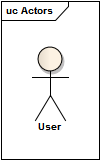
\includegraphics[scale=1]{../ea_files/generatedImages/Simulator/Actors.png}
			\caption{Actors of simulation tool.}
			\label{fig:actors}
		\end{figure}
		
		\begin{figure}[!hbtp]
			\centering
			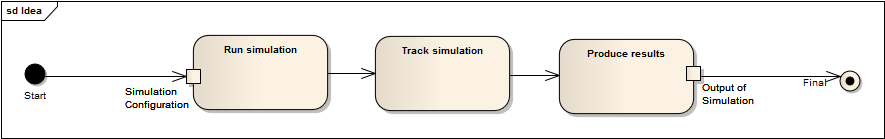
\includegraphics[width=\textwidth]{../ea_files/generatedImages/Simulator/Idea.png}
			\caption{Idea, happy path of a simulation.}
			\label{fig:idea}
		\end{figure}
	
		\begin{figure}[!hbtp]
			\centering
			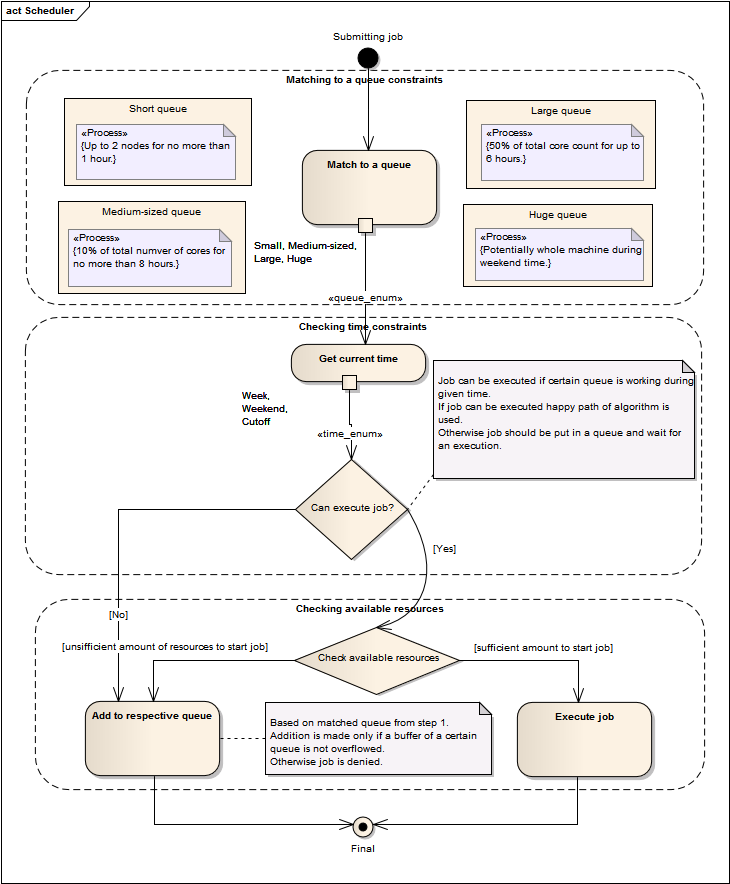
\includegraphics[width=\textwidth]{../ea_files/generatedImages/Simulator/Scheduler.png}
			\caption{Scheduling algorithm of a simulation tool.}
			\label{fig:scheduler}
		\end{figure}
	
		\begin{figure}[!hbtp]
			\centering
			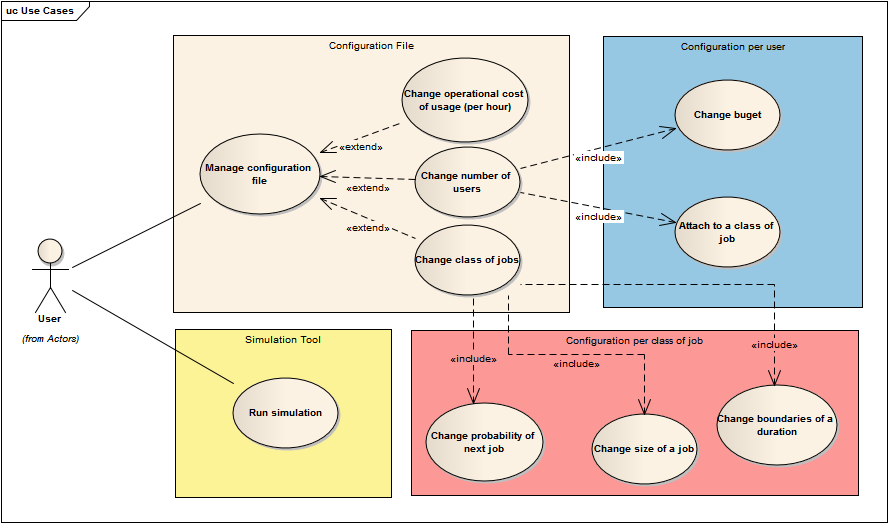
\includegraphics[height=\textwidth, angle=90]{../ea_files/generatedImages/Simulator/UseCases.png}
			\caption{Use cases for simulation software.}
			\label{fig:use-cases}
		\end{figure}
\end{appendices}

\printglossaries

\end{document}
